\section{Preliminary Evaluation}\label{sec:evaluation}
In this section, we discuss some preliminary evaluation results about the ReCapture framework. We use one laptop as the central master of the ReCapture framework and two Google Nexus S smartphones. The Nexus S smartphone's specifications are shown in Table~\ref{tab:nexus}. In addition, Fig.~\ref{fig:exp} displays the experiment environment that two Nexus S smartphones connect to a laptop as the central master.

\begin{table}
\centering
\caption{The Nexus S smartphone specifications}
\begin{tabular}{ll}\toprule
CPU & 1 GHz Cortex-A8 \\
GPU & PowerVR SGX540 \\
RAM & 512MB \\
Storage & 8GB \\
Sensors & Accelerometer, gyro, proximity, compass \\
GPS & Yes, with A-GPS support\\
OS & 4.1.2 (Jelly Bean) \\\bottomrule
\end{tabular}
\label{tab:nexus}
\end{table}

\begin{figure}
\centering
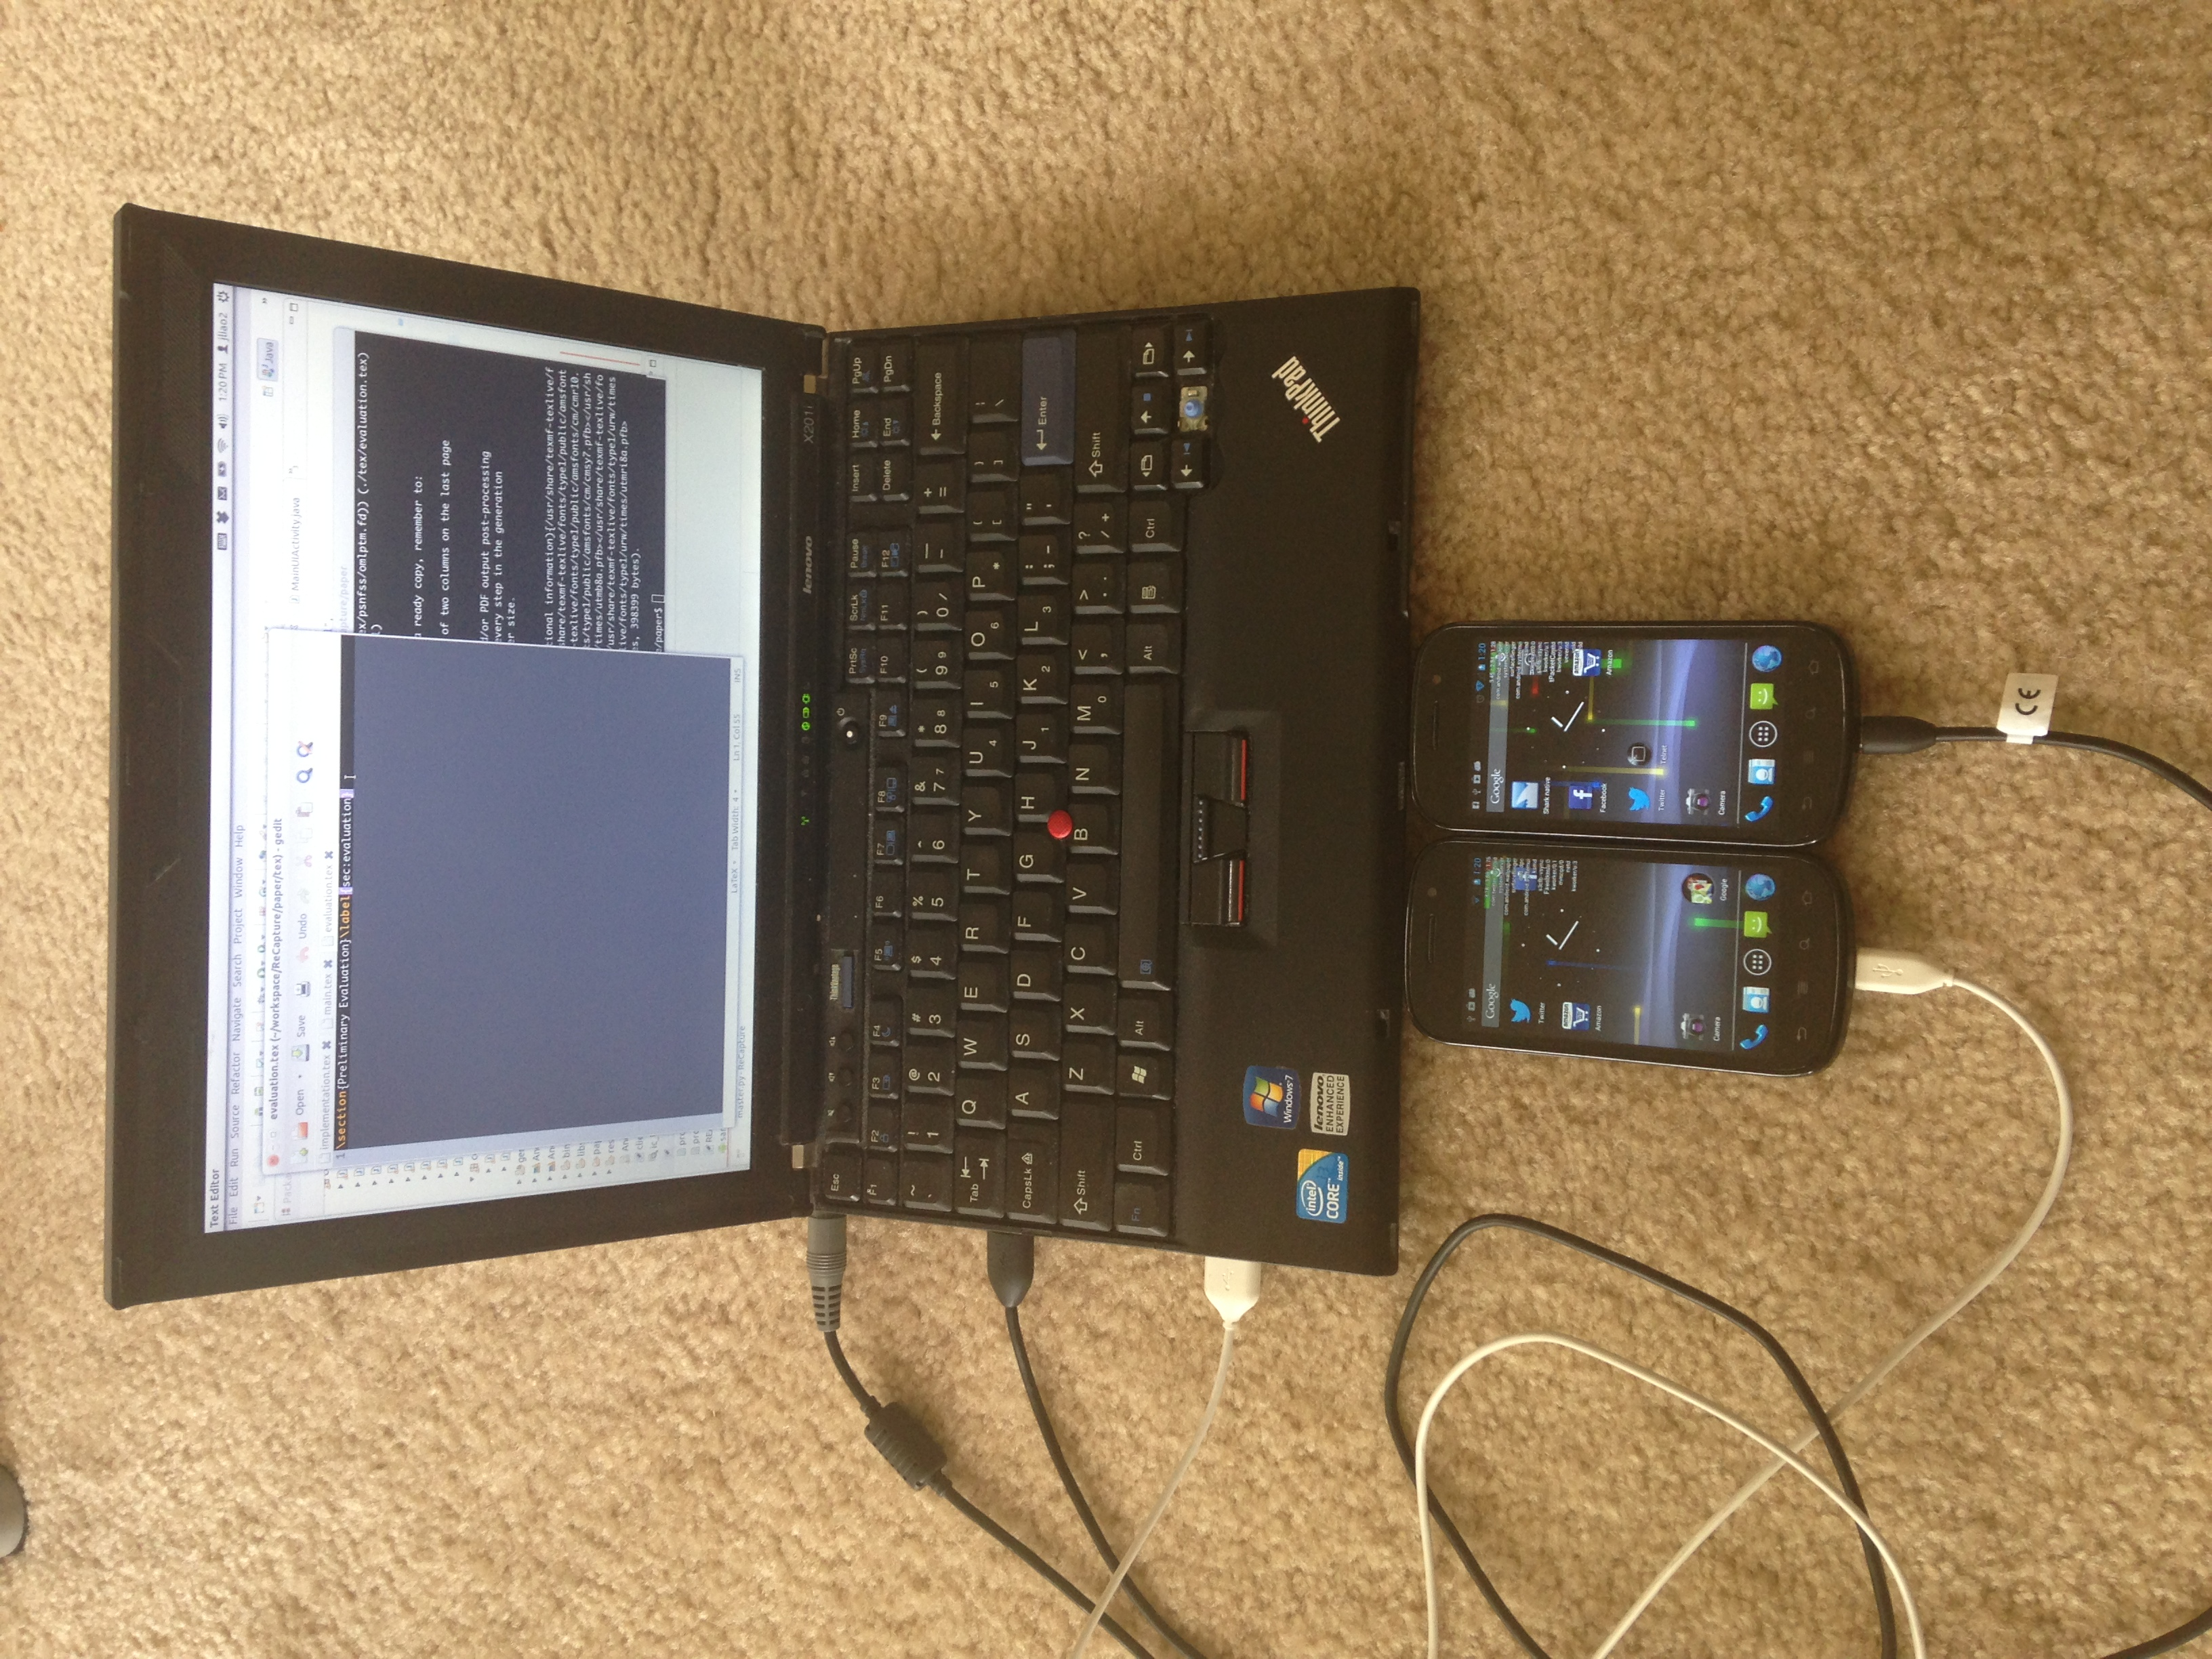
\includegraphics[width=0.45\textwidth]{figures/experiment.jpg}
\caption{Experiment setups}
\label{fig:exp}
\end{figure}

We prepare a sample activity log in the Table~\ref{tab:log}, which we repeat the execution of facebook, gmail, twitter and amazon app and each of the app will last $5$ seconds. After a round of execution, we collect the screen actions issued to the devices and the statistics is shown in Table~\ref{tab:screen}. As we can see, the most active screen operations are navigations, touch and motion. If you are using facebook, you may swipe up and down to see new feeds or use the navigations to jump into to chat. It is also frequent that you may see a picture and you click the picture, then you change the orientation of the phone to see the picture, so the motions activities also introduces about $10$ percent of the total screen actions. Further more, Fig.~\ref{fig:master} records a screen snapshot of the central master. Once the master receives activity hook message, it will start generating the screen action code to the device.

\begin{figure*}
\centering
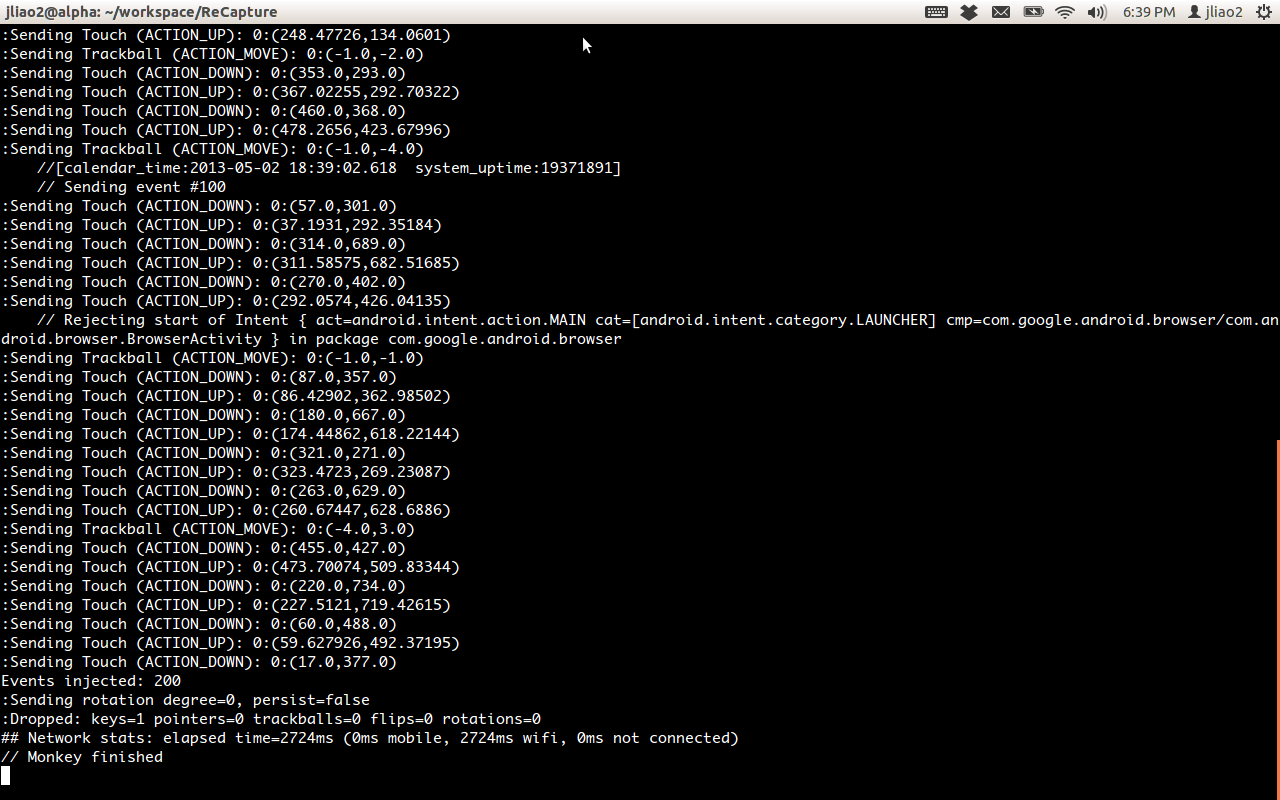
\includegraphics[width=0.8\textwidth]{figures/master.png}
\caption{The central master screen snapshot}
\label{fig:master}
\end{figure*}

\begin{table}
\centering
\caption{The sample activity log}
\begin{tabular}{ll}\toprule
activity event & duration (ms) \\\midrule
facebook & $5,000$ \\
gmail & $5,000$ \\
twitter & $5,000$ \\
amazon & $5,000$\\\bottomrule
\end{tabular}
\label{tab:log}
\end{table}

\begin{table}
\centering
\caption{Screen actions results}
\begin{tabular}{ll} \toprule
Screen Action Category & Percentage \\\midrule
Touch & 15\% \\
Motion & 10\% \\
Traceback & 2\% \\
System Keys & 0\% \\
Navigations & 25\% \\
Major Navigations & 15\% \\
App Switch & 2\%\\
Flip & 2\% \\
Others & 10\% \\\bottomrule
\end{tabular}
\label{tab:screen}
\end{table}

On the other hand, we are interested in the central master's capability to receive large amount of screen action requests. It is important because the central master could become the bottleneck of the system in a large scale environment. In this experiment, we test how well the central master can answer the request from the device by sending $1,000,000$ request in multiple thread concurrently to the central master. Fig.~\ref{fig:time} shows the results, as we can see, $90\%$ of the request can get response within $2$ms, so the delay of the system is very small. It is safe to say that the central master should not become a bottleneck of the whole system.

\begin{figure}
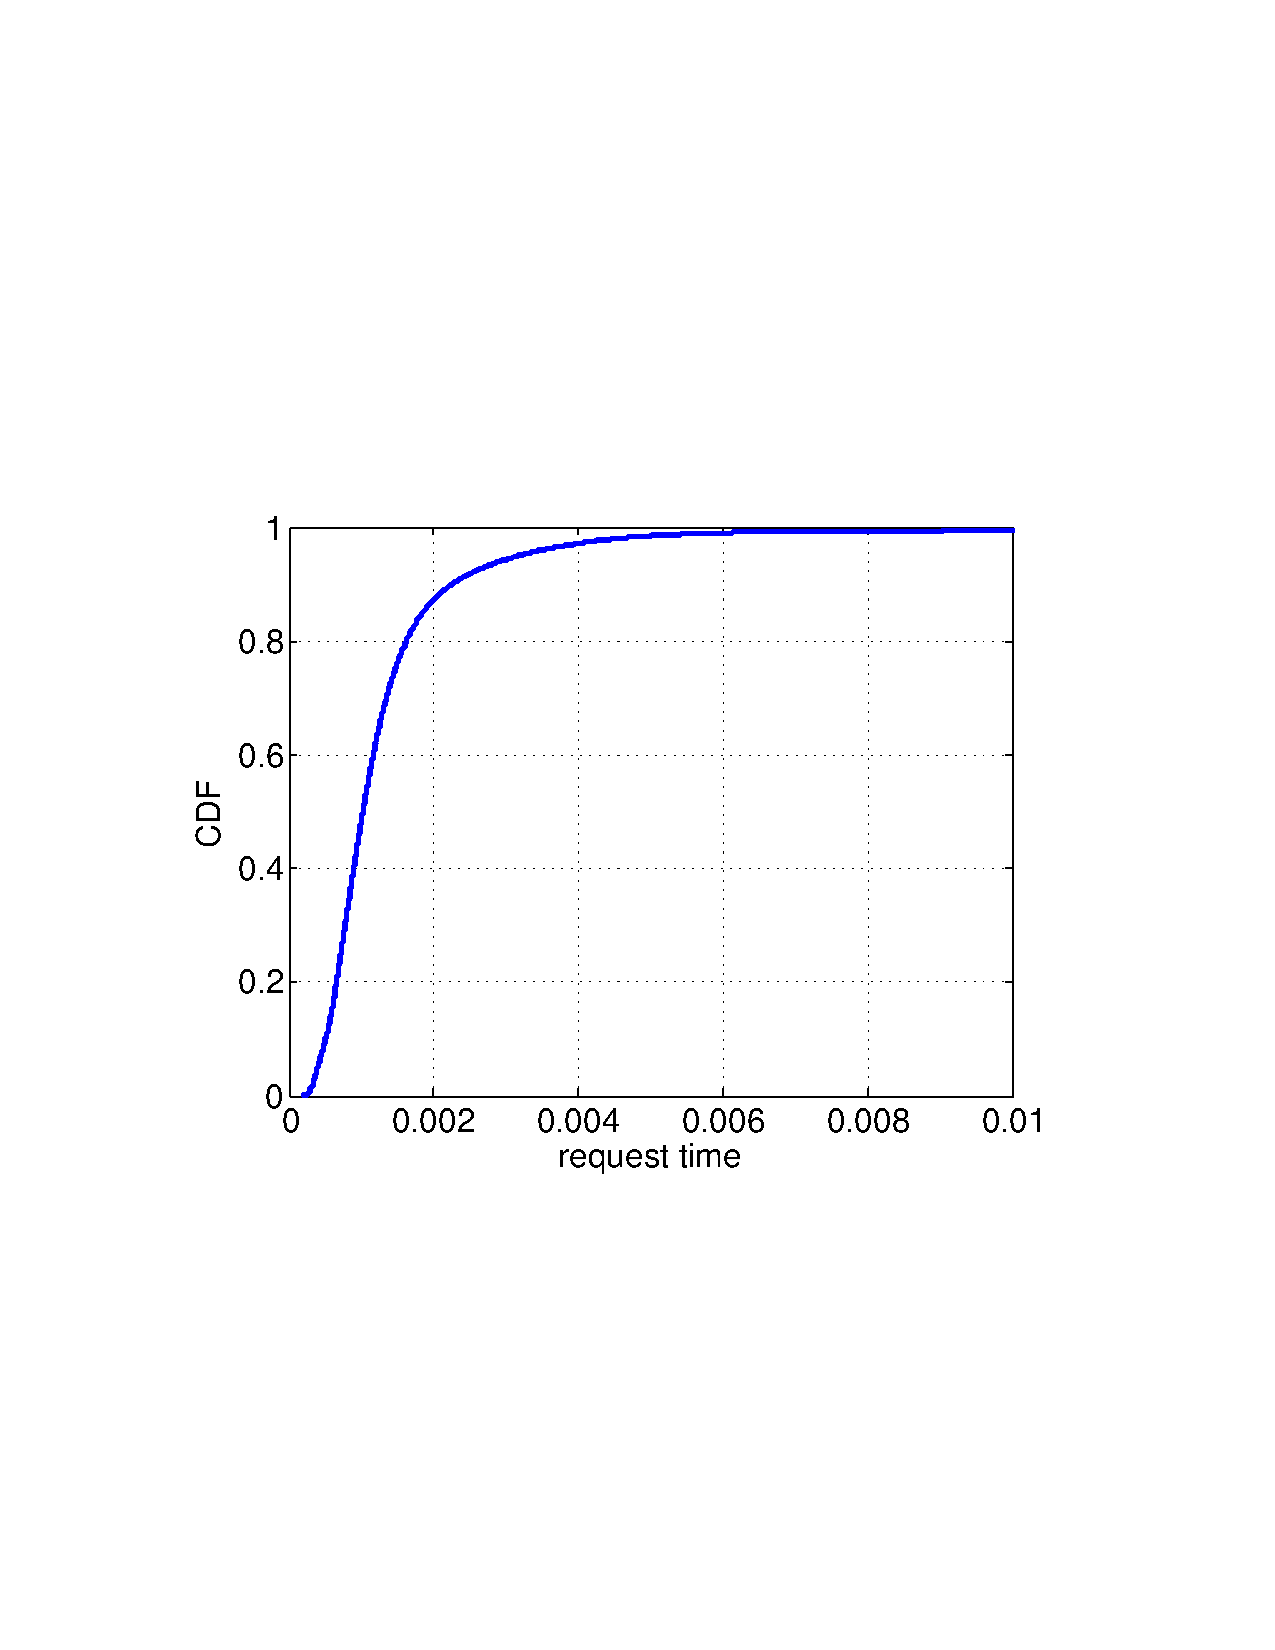
\includegraphics[width=0.45\textwidth]{figures/time.pdf}
\caption{Time response of central master}
\label{fig:time}
\end{figure}
